% !TeX root = ./proposta-pytorch.tex
\documentclass[a4paper,12pt, brazil]{article}

% --- PREAMBULO ---
% 1. Load Used Packages
% █▀█ █▀█ █▀▀ ▄▀█ █▀▄▀█ █▄▄ █   █▀▀
% █▀▀ █▀▄ ██▄ █▀█ █ ▀ █ █▄█ █▄▄ ██▄
%::::::::::::::::::::::::::::::::::::::::::::::::::::::
%                      CORE SETUP                      
%                Document-Wide Settings                
%......................................................
\usepackage[utf8]{inputenc}	         % Input encoding: Assumes UTF-8 text editor
\usepackage[T1]{fontenc}             % Output enconding: 8-bit, for better glyph support
\usepackage[margin=2.5cm]{geometry}  % Set page margins
\usepackage[brazil]{babel}           % Language-specific settings

%::::::::::::::::::::::::::::::::::::::::::::::::::::::
%                       GRAPHICS                       
%                Generate/Import Images                 
%......................................................
%% NATIVE PROGRAMMATIC DIAGRAMS & PLOTS
%\usepackage{tikz}		        % Create vector graphics programmatically
%\usetikzlibrary{arrows.meta}	% Additional arrow styles
%\usepackage{pgfplots}		    % Tool for creating function plots and charts
%\pgfplotsset{compat=1.18}	    % Enforce version 1.18 for consistency

% EXTERNAL IMAGE MANAGEMENT
\usepackage{graphicx}		    % LaTeX standard for including external image files

%::::::::::::::::::::::::::::::::::::::::::::::::::::::
%                    MATH PACKAGES                     
%......................................................
% AMS (American Mathematical Society)
\usepackage{amssymb} 	% AMS's package for mathematical symbols
\usepackage{amsmath}	% AMS's package for mathematical typesetting
\usepackage{mathtools}  % Extends amsmath's functionalities (i.e.: a superset)
\usepackage{amsthm}    	% AMS's package for creating theorem-like environments


% LOADED LAST TO AVOID DEPENDENCY ERRORS
%::::::::::::::::::::::::::::::::::::::::::::::::::::::
%                     BIBLIOGRAPHY                      
%                   Manage References                   
%......................................................
\usepackage[
	backend=biber,	% Use Biber backend (more powerful than BibTex)
	style=ieee,     %
	sorting=nyt     % 'nyt' stands for name, year, title
]{biblatex}

%::::::::::::::::::::::::::::::::::::::::::::::::::::::
%                     FINALIZATION                      
%    Packages That Patch Others. MUST BE LOADED LAST    
%......................................................
\usepackage{hyperref}	% Add hyperlinks to references, ToC and URLs
\hypersetup{
	colorlinks=true,	% true: colored links; false: boxed links
	allcolors=NavyBlue,	% Set all link types to a single color
}

% 2. Configure Project-Specific File Paths
\addbibresource{referencias.bib}
\graphicspath{ {./imagens/} }

% --- START OF DOCUMENT ---
\begin{document}
    % --- TITLE BLOCK ---
    % !TeX root = ./proposta-pytorch.tex
\begin{center}
	\begin{figure}[h!]
		\centering
		
\includegraphics[height=1.5cm]{logoICMC.png}
	\end{figure}

	\rule{0.95\textwidth}{1.5pt}

	\vspace*{2mm}

	{AEX \par}

	\vspace*{1mm}

	{\large Trabalho 1\par}

	\vspace*{3mm}

	{\Large\textbf{Pytorch do Zero}\par}
	
	\vspace*{3mm}

	{\large\textbf{\emph{Métodos da Bisseção, Newton-Rhapson e das Secantes}}}

	\vspace*{8mm}

	\begin{tabular}{rrcl}
        Docente Responsável: & Prof. Dr. Lucas Pascotti Valem \\
        Alunos: & \\
        & Amanda Araújo & -- & XXXXXXXXXX \\
		& Cody Stefano Barham Setti & -- & 4856322 \\
		& Ian Cavalcanti de Holanda Bezerra & -- & XXXXXXXXXX
	\end{tabular}

	\vspace*{8mm}
	
	{\normalsize \today\par}

	\vspace*{2mm}

	{\normalsize São Carlos, SP, Brasil\par}

	\vspace*{2mm}

	\rule{0.95\textwidth}{1.5pt}
\end{center}
\vspace*{5mm}

    
    \begin{figure}[h]
        \centering
        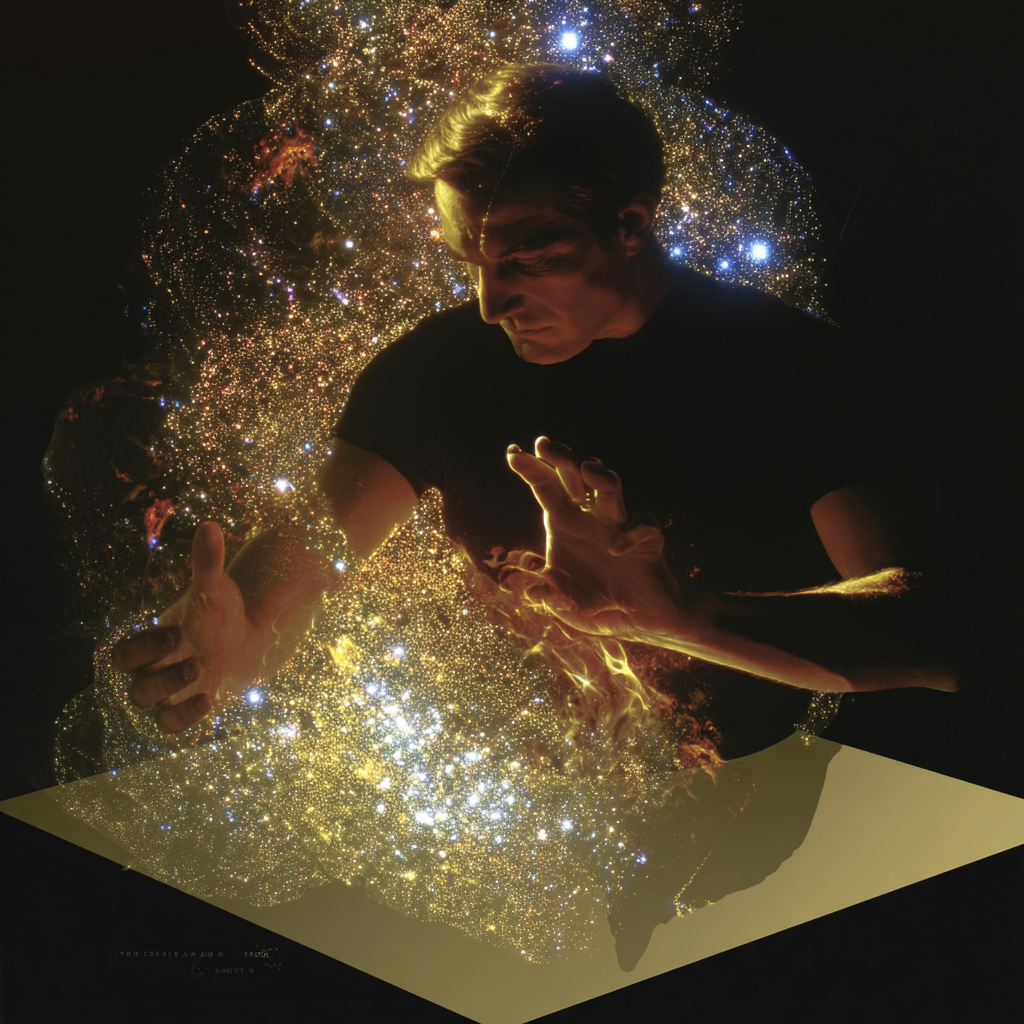
\includegraphics[width=0.6\textwidth]{imagem-de-capa.png}
    \end{figure}
    
    \newpage
    
    % --- ARTICLE BODY ---
    \section*{Proposta da AEX}
    
    \section*{Aulas}
    \begin{itemize}
        \section*{Bloco 1 - IA do Zero}
        \item Video 1 - Introducao e Revisao
        \begin{itemize}
            \item Introducao ao curso
            \item Machine Learning, introducao ao problema do pipeline, complexidade, informacao. 
            \item Enviorment, bibliotecas, colab. Configurando maquina.
        \end{itemize}
    
        \item Aula 2 - Revisao de Conceitos Nessesarios.
        \begin{itemize}
            \item Revisao Matematica, Funcoes (Rn em Rn) Derivadas Parciais, Gradiente. 
            \item Parte 1: Gradientes e Backprop. 
        \end{itemize}
            
        \item Aula 3 - Torch Autograd Sistem do zero.
            \begin{itemize}
                \item Parte 2: Model class, exemplo seno, primeiro MLP, e levando conceitos a Torch, torch optim. 
                \item Parte 3: O que eh uma GPU, activation functions, Revisao conceitos. 
            \end{itemize} 
        
        
        \section*{Bloco 2 - Arquitetuas de NN}
        \item Video 4 - Introducao as Arquiteturas de NN.
        \begin{itemize}
            \item Torch NN.module e resolvendo MNIST (CPU, GPU). 
            \item Problemas comuns Parte 1: Overfitting, Exploding Gradients, Vanishing Gradients
            \item Problemas comuns Parte 2: Layer Normalization, Batch Normalization, Shuffle correspondance.
        \end{itemize}
        
        
        \item Video 5 - Mais Arquiteturas de NN e Pratica.
        \begin{itemize}
            \item CNNs.
            \item RNN.
        \end{itemize}
        
        \item Video 6 - Pratica.
        \begin{itemize}
            \item Pratica. Kaggle to Solved NN.
        \end{itemize}
    
        \section*{Bloco 3 - Dados e Praticas de Producao}
        
        
        \item Video 7 - Embeddings e Tranfer Learning.
        \begin{itemize}
            \item Embeddings
            \item Modelos Pre-Treinados. (LLMs, TTS, STT, Stable Difuision)
            \item Pontos Importantes de modelos grandes em GPU.
            \item Tranfer-Learning
            \item Finetuning
        \end{itemize}
        
        
        \item Video 8 - Dados: Extracao, Contaminacao, Criacao. (ChemAI)
    
        
        \item Video 9 - Infra-Estrutura para IA.
        
        \item Video 10 - Colocando IA em Producao.
    
    \end{itemize}
    
        
    \section*{Material}
    \begin{itemize}
        \item Bloco 1 \\ Andrej Karpathy - zero to hero(2 Primeiros videos)\cite{karpathy}\\ https://www.youtube.com/playlist?list=PLAqhIrjkxbuWI23v9cThsA9GvCAUhRvKZ
        
        \item Bloco 2 \\ MIT - AI course\cite{mit_ai} \\ MIT 6.S191: Introduction to Deep Learning\cite{mit_deep_learning}
        
        \item Bloco 3 \\ Praticas de AI, Material Proprio \\ AI-Chem, Zero to hero aulas 3-5.
    
    \end{itemize}    
    
    \section*{Horas - AEX}
    
    Tempo de preparar as Material: 5h por aula.\\
    Tempo de preparar as Video: 4h por aula.\\
    Tempo de aula: 30-45min por aula.\\
    \textbf{Total de aulas: 10 Videos. 20 Semanas.}\\
    Total = 10 * 0.8 + 10 * (5h Para Preparar Material) + 10 * (4h Para Preparar Video) = 98 Horas total.
    
    % --- BIBLIOGRAPHY ---
    \printbibliography
\end{document}